\documentclass[conference]{IEEEtran}
\IEEEoverridecommandlockouts
% The preceding line is only needed to identify funding in the first footnote. If that is unneeded, please comment it out.
\usepackage{cite}
\usepackage{amsmath,amssymb,amsfonts}
\usepackage{algorithmic}
\usepackage{graphicx}
\usepackage{textcomp}
\usepackage{xcolor}
\usepackage{pgfplots}
 
\pgfplotsset{compat = newest}

\def\BibTeX{{\rm B\kern-.05em{\sc i\kern-.025em b}\kern-.08em
    T\kern-.1667em\lower.7ex\hbox{E}\kern-.125emX}}
\begin{document}

\title{Oblivorian Vulnerability Scanner and Simple Vulnerability Scanning and Checking\\
}

\author{\IEEEauthorblockN{Nicholas Garrett}
\IEEEauthorblockA{\textit{Computer Science} \\
\textit{Idaho State University}\\
Pocatello, Idaho, United States \\
garrnic3@isu.edu}
}

\maketitle

\begin{abstract}
Computer system vulnerabilities are far from uncommon and in this increasingly computer-driven world, patching these vulnerabilities is becoming more and more important.  In response to the growing number of available security flaws, vulnerability scanning systems have been implemented and made available to scan phones, personal computers, and an increasing spread of devices to detect these flaws--some even work to repair these flaws.  

Described in this paper is a small-scale vulnerability scanning system meant to search a target computer system for some simple exploitable security points.  This program, written in mainly the Python3 programming language and dubbed ``Oblivorian'', is designed to run in a mainly educational environment, mainly intended to explore existing functionality of vulnerability scanners.  However, this program does act to explore some of the actual mechanics used in commercial-grade scanners.
\end{abstract}


\section{Introduction}
When the first commercially available personal computer, the Kenbak-1, was released to the 
public in 1971\cite{b1}, the concept of computer viruses was only that—a concept.  It was not until the spread of the Creeper Virus of that same year that the need for cyber security became evident.  Prior to Creeper, popularly known as the first computer virus\cite{b2}, the practical need for implementations to avoid vulnerabilities only contained bug-fixing and avoiding system errors.  However, with the rising popularity and prevalence of computer viruses being spread from system to system, the importance of maintaining security and preventing cyber attack is rising as well.  \\

	In this paper, I describe a software system I have built intended to detect common exploitable issues easily detectable on a computer system.  I will also explain these possible exploits and how they pose issue and threat to computer systems.  Each of the exploits I will describe—or methods to reach exploit—are useful to an attacker intending to gain access to a computer system.  \\
	

\section{Oblivorian}
As previously described, vulnerability scanning programs have become more and more important as the number of cyber attacks made against computer systems has been increasing an ever-increasing rate.  Often, the actual implementations and methods used by scanning software seem vague and unconvincing\cite{b10}.  In other words, how vulnerability scanning programs operate is very often hidden from the user; what a user sees is only the end determinations and recommendations made by the program.

So, in order to greater appreciate the availability of scanning software and understand the algorithms used in those programs, I have implemented a software program to try and actually check for some of these vulnerabilities.  The software program I have built to solve some of these issues in cybersecurity is called Oblivorian.  \\

	The name ``Oblivorian'' is derived from the two key words of ``Oblivion'' and ``Orion''.  ``Oblivion'', as defined by Merriam-Webster, is ``a state marked by lack of awareness or consciousness''\cite{b11}.  This base word was chosen as it describes the lack of knowledge on the topic of vulnerabilities and scanning, and general ignorance prior to actually building the system.  The second base word, ``Orion'', was chosen for a different reason.  The constellation Orion is also known by another name: the hunter.  This software program is intended to hunt for vulnerabilities of a target system.  
	These two base words describe the hope of Oblivorian: to hunt for vulnerabilities of a system and destroy the ignorance of how cyber-threat scanning works. \\
	
	Past the etymology of Oblivorian, the actual implementation of such a system is significantly more important than the system itself.  Oblivorian is presently written in Python3 due to the high-level of control available in such a language.  Python3 is often looked down on by programmers due to how high-level it is in terms of control--it is so far away from systems programming that there can be little trust in it serving as an effective scanner of vulnerabilities.  This is understood, and given time, Oblivorian is expected to be implemented, at least partially, in a lower-level language--a language like C. \\
	
	This software program is designed to scan a computer system for some of the simple vulnerabilities seen.  And, as with almost any software system, Oblivorian is a continuously changing software program designed to change and improve over time.  Hopefully, given enough time, this program will be able to scan for more advanced and difficult software vulnerabilities beyond some of the simple surface-level vulnerabilities is is currently capable of checking.  Of  course, it is unfortunately limited by my abilities in programming and by the extent of my understanding in cybersecurity principles.  As I become more competent and knowledgeable about cybersecurity and vulnerability scanning principles, I will add to Oblivorian and hopefully build it into a competent scanning system.  \\
	
	Unfortunately, Oblivorian is only designed to operate on a Linux machine.  This is mainly due to some of the slight differences in how commands are supposed to be run between the two systems.  While there is some OS checking incorporated in Oblivorian to allow for slightly different scripts or commands to be run depending on the OS, not all the functions incorporate this checking, so some features will either malfunction or might even outright fail on a Windows system. \\  
	
	Throughout the extent of this paper, I will describe various generic vulnerabilities that are easy to check and how Oblivorian works to fix or detect these vulnerabilities.  Of course, not all of the points discussed will be vulnerabilities per se, for example the System Information scanning.  However, they all are involved in vulnerability scanning, or the availability of such information can help an attacker to better attack or gain access to a system. 
	
	Oblivorian git repository: https://github.com/codemaxx1/Oblivorian.git\\
	

\section{Port Scanner}
	Internet ports are an important part of connecting a computer system to the outside world. Through them information and data can be both sent and received across the internet.  Through this, a personal computer in Japan, for example, is capable to sending data to another system anywhere else in the world.  
	
	However, while network ports must be open in order to connect to the outside world, this is a double-edged sword: every open port is a potential vulnerability that an attacker could exploit.  An attacker needs only to gain access to a port and they can then possibly get information about your system and open doors for the execution of malicious software.  At this point, an attacker effectively has control of the targeted system. \\
	
	Often, specific ports will be opened by a process to connect to some remote servers.  An example of this is the VMware process, which listens on port 902\cite{b8}. This service is not always running and not all computer systems even have VMware installed. So, logically, unless some program or process opens and listens to this port, it will by default remain closed.  When a process does open and begin listening on a port, it will open that port for as long as the process is running. However, just because some process opens a port, that does not inherently mean that it is actively listening to that port.  It is not too uncommon for ports to be left open for no reason--it is these ports in particular that can pose a security risk.  Therefore, in order to ensure our computer system is more secure than otherwise, we should make sure that only ports we want to be open remain so, and all non-actively used ports are closed. 

	However, what defines a used verses an unused port?  Simply put, a used port is one in which the daemon, a program that runs in the background without input from the user, is still listening on a port.  Therefore, by the logical conjugate, we can say that unused ports are those in which no daemon is listening for incoming traffic.\\ 
	
	Our first thought might be to simply close all the ports we do not want to use.  This would prevent attackers from retrieving information about our system.  Logically, such an action would improve the port-security of the defending system; it would also act to reduce the available vulnerabilities an attacker can use in their attempts to control a target system.  However, this impulsive action could lead to necessary ports being closed.  
	
	Suppose we close the ports necessary for HTTP or HTTPS (80 and 443 respectively), suddenly we would find that internet browsing programs no longer work, as HTTP and HTTPS are important in transferring the data used in internet browsing. 

	Thus, we can see that closing ports without first seeing what they do or closing ports often used, can lead to the processes using those ports to malfunction or fail.  Therefore, we must be careful not only to close unused ports, but also to not close open ports that are used frequently.\\
	
	Instead of automatically closing open ports when they are found, if we list the ports and give to the user the option of what ports to close, giving to them an explanation of what the purpose of these ports are, the risk of closing ports best left open can be decreased and control can be put into the hands of the user.  
	
	Following this plan, it is quite possible that the list of open ports may be quite large.  For example, Mac-OS websites state that as about 132 ports are open by default on many Apple services.  To improve user experience, it would be more convenient to somehow filter through ports that should be closed, only leaving ports with an active owner up to the user to close if wished.
	
	Thus, Oblivorian’s scanning feature scans through port numbers 1 through 65535.  The method of searching for open ports is through attempting to connect to the ports in iterative sequence; if a connection is able to be made, then that indicates that a service is listening on that port.  So, Oblivorian adds each port where a connection could be made into an array and asks the user whether or not to terminate all processes listening-in on that port.\\


\section{System and Processor information}
Accessing system information on a target computer system is important in scanning for vulnerabilities.  Something as simple as determining a computer's Operating System can help attackers to narrow down and target particular vulnerabilities.  
For instance, Windows XP has software vulnerabilities that are specific to it, whereas Windows 98 has its own OS-specific vulnerabilities--relatively few of these assailable points are shared between the two systems compared to the number of attacks able to be made to exclusively a single Operating System\cite{b9}.  

This is not an offense against Windows XP or Windows 98 in particular, every Operating System has its own set  of vulnerabilities--it is almost impossible to completely remove the presence of hackable points.  Rather, this should go to explain and demonstrate that vulnerabilities exist that are not shared among multiple operating systems.  

If an attacker is able to narrow down what  type of system they are attacking--even if the exact operating system is still indeterminable--they can more specifically and actively narrow down the available software attacks that can be made against the system.  If the exact operating system, release, version, processor, or even if it is a 64 or 32 bit machine can be determined, an attacker can better and more accurately narrow-down the list of attacks they should make that are the most likely to break the target systems countermeasures and gain access to the system.\\

In March 2018, researchers at Ohio State University in the United States announced a method to breach the internal security for an Intel CPU\cite{b16}.  In this published exploit, researchers described a method through which an attacker is able to gain access to the system and can both read and write memory.  The researchers who published this vulnerability dubbed it ``SgxPectre''\cite{b15}.  

This is just one example of a hardware-specific vulnerable attack that can be made against a system if the information can be determined.  

\subsection{Determination of processor by mathematical calculations}
The issue of a processor-specific vulnerabilities being used against a specific computer processor is a much more difficult issue to protect against than Operating System vulnerabilities\cite{b12}.  However, it is luckily also quite difficult to determine what processor a target system is using.   

Unfortunately, research is showing that while it is difficult to identify the processor of a system without having access to that level of information, it is not impossible.  One method of determining what processor a system is using is through the actual calculations made by that processor. \\

Due to the physical makeup of different processors, as well as the algorithms used for mathematical calculation, the return they give for mathematical approximations are variant.  It is in the nature of their construction that the algorithmic and approximation errors will vary by a small degree from the exact solution for some mathematical calculation\cite{b17}.  For example, if one were to calculate \(\sqrt{2}\) on some computer system, an approximation for that solution would be returned.  If then, one were to compare the calculated return for \(\sqrt{2}^2\) and 2, the two would not be equivalent\cite{b13}.

Taking advantage of this variance, we can get a reasonably accurate idea of what specific processor a system uses.  A practical implementation of such a method follows: if we define some mathematical operation, then certain expected values will be returned by mathematical operations.  Further, each of the values returned will be slightly different depending on each processor chip.

\begin{figure}
\begin{center}
\begin{tabular}{ |p{2cm}||c|c|c|| }

 \hline
 Processor	& \(sin(10^{10} \pi_1)\) & \(sin(10^{17} \pi_1)\) & \(sin(10^{37} \pi_1)\)\\
 \hline
 IPHONE 3G   	& 0.375...		& 0.423... 	&  -0.837 \\
  AMD 32 	&  0.375... 	& 0.424... 	& -0.837 \\
 AMD 64 		&  0.375... 	& 0.424... 	&  0.837 \\
 ATOM    		& 0.375... 	& 0.423... 	&  -0.832 \\
 INTEL DC 	& 0.375...		& 0.423...		& -0.832 \\
 MIPS 12000	& 0.375...  	& 0.423...   	& -0.832 \\
 dsPIC33 		& 0.81...  		& 0.62... 		& -0.44  \\
 \hline 
\end{tabular}\\
\caption{Float calculations for various processors\cite{b13}.} \label{Table 1}
\end{center}
\end{figure}
Table 1 shows some examples of how mathematical calculations differ slightly for different processor families.  \\

In order to test this principle--to the limited degree of available and accessible data--Oblivorian includes a C script which runs the calculations of a few trigonometric functions: \(sin(10^{10} \pi), \, sin(10^{17} \pi)\), and  \(sin(10^{37} \pi)\) to try and determine the processor family of the running system.  
Unfortunately, the degree to which this calculation narrows down the specific processor is still incomplete, as limited information about the actual returns for such calculations is available.  

	The only information that could easily be found is the data listed in Figure 1, which quite obviously does not encompass a particularly wide range of processors that can be identified.  Thus, unfortunately the script included in Oblivorian to test based on processor float calculations is fatally lacking in the range of processors it can determine. \\

\section{Password Cracking}
Often, system security is thought of as exclusively the low-level operations and vulnerabilities through which an attacker may gain access to a system.  However, not all attacks require increasingly more complex and complicated attacks in order to breach a system's defenses.  Instead of beating relentlessly against the strong points of a system, the points already defended, would it not be rather practical to direct efforts and resources to attacking the weakest point of security?  Of course.

In the enforced chain of system security, the weakest link is almost invariably the user.  If the user can be manipulated into inadvertently granting access of their machine to an attacker, then time potentially wasted in attacking the system directly can be used much more efficiently.  \\

This nearly invisible piece of system security of which the user holds control is the password.  In order to properly defend a system, the password must be sufficiently difficult to break that attackers could not guess it in any reasonable amount of time.  The way to do this is by preventing the two main password cracking systems: brute force and word list guessing.

\subsection{Brute Force}
Brute force guessing of passwords is the easier of the two to implement, though it is also the least efficient.  By randomly or alliteratively guessing all possible combinations of characters, the correct password will eventually be guessed.  However, this method is incredibly inefficient; the number of checks required to eventually guess the correct password grows exponentially with each additional character following a function of \((available characters)^{characters in the password}\)\cite{b23}, a visual representation of this is shown in Figure 2.  As we can see from the figure, an exponential spike in 
\begin{figure}
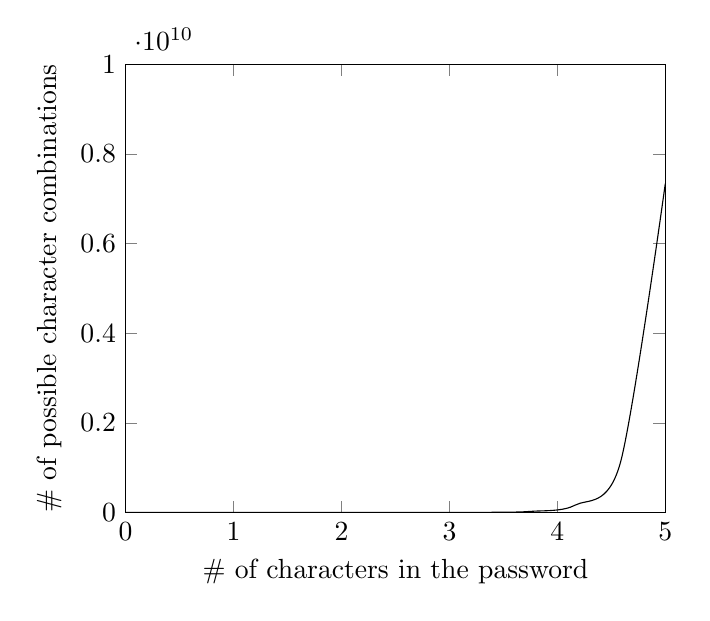
\begin{tikzpicture}
    \begin{axis}[
    	xmin = 0, 
    	xmax = 5,
   	ymin = 0, 
   	ymax = 1*10^10,
   	xlabel={\# of characters in the password},
   	ylabel={\# of possible character combinations},
   	 ]
        \addplot[smooth] {(126-32)^x};
    \end{axis}
\end{tikzpicture}
\caption{Exponential growth of possible character combinations for an inputted word} \label{figure 2}
\end{figure}

Thus, running Brute force password crackers can take an incredibly long time.\\

Oblivorian is implemented with two brute force password cracking scripts.  The first of these two is a randomly-generating string guesser.  It operates, as the name implies, by randomly selecting a character from the full list of characters, including capital letters, lowercase letters, numbers, and symbols.  By building an array of randomly generated characters and converting that array into a string, the ``guess'' can be made.

The second of the brute force algorithms in Oblivorian is an iterative character guesser.  This password guesser, as opposed to the randomization algorithm, builds an array and simply iterates through each and every possible character combination.  For example, in a length 4 password, the first array would be [`` '', '' '','' '', '' ''], then the next character array, or string, would be [`` '', `` '', `` '', ``!'' ], and so forth until it had iterated through every single possible character.

However, because of the simple nature of it running in such a high-level and low priority language, these two scripts run much slower than if they were to be in a smaller, faster program.  On a properly streamlined program and in a lower-level language, over 11 million keys can be tested each second, as tested on an Intel I5-6600K\cite{b23}.  Though, this is based on the estimation that most of the attack systems resources are allocated to the password cracking, and the upper bound of keys able to be tested is held by the processor's cycle speed.


\section{Passwords}
As described in the previous section, passwords are an incredibly important piece of maintaining security for a system.  The more advanced and complicated a password is, the more time it will take for a brute force password guesser to determine your password.  This is great; if you just need a longer password to evade algorithms, then it shouldn't be too difficult to simply have a password of the maximum size that would take more time to break than has passed in the Event Horizon of a black hole\cite{b24}. 

While this may seem like the best way to ensure a system is password-protected, there is a glaring security flaw that implicitly must reside in local passwords for a system.  No matter how short or long a password is, it must be stored somewhere.  \\

In most Linux systems, the location where passwords and user information is stored is in the ``/etc/shadow'' and ``/etc/passwd'' respectively.  This is the most popular authentication system used for Linux systems, and has become the standard\cite{b25}.  \\

The shadow file, located at ``/etc/shadow'', is populated with information relating users to their passwords, including the actual password themselves.  Luckily, the passwords stored in this file are all hashed, but the hash data is still held in the file.  
Due to the importance of maintaining the security of such an important file, the shadow file can only be accessed by a Super User authority.  So, only authorized users should be able to access the information stored in that file.

If an authorized user were to print the information from this file, the output will follow a clearly-organized schema.  Each line in the Shadow file coincides to a different user, and is a colon-separated list of values of the format: [username]:[encrypted password]:[last password change]:[minimum password age]:[maximum password age]:[warning period]:[inactivity period]:[expiration date]:[unused] \cite{b25}, an example for what a line in this shadow file might look like follows: ``linuxize:\$6\$zHvrJMa5Y690smbQ\$z5zdL...:18009:0:120:7:14::''.\\

\subsection{Username}
The username string is, as the name implies, the user account that exists on the computer system.  It is the account a user is logged-in as, and very rarely has advanced permissions. \\

The second field contains the encrypted password.  It follows the \$encryptionType\$salt\$hashedPassword method, which is itself a \$-separated list of values representing the type of encryption used, the salt, and the hashed password.

There are several different types of encryption methods that can be used.  As such, the value of this field is incredibly important in the process of actually decryting the hashed password.
The algorithms for hashing are as follow:
\begin{itemize}
  \item \$1\$ \(\rightarrow\) MD5 
  \item \$2a\$ \(\rightarrow\) Blowfish 
  \item \$2y\$ \(\rightarrow\) Eksblowfish 
  \item \$5\$ \(\rightarrow\) SHA-256
  \item \$6\$ \(\rightarrow\) SHA-512 
\end{itemize}

The second field in password is the salt.  A salt is a small string that is inserted in the hashing function, which makes the decryption of the password much more complicated\cite{26}.

Following the salt, the third field in password contains the encrypted password text, which is the hashed return made by passing the password and salt through whichever encryption method was used.  The length of the hashed password depends on the method used to hash the function.  

However, a important note is that the field may contain a single character: a ``!'' or ``*''.  The presence of either of these two characters indicate that the account is locked, meaning the user is not able to gain access to that account.  Often, the ``root'' account will have this password setting, as the user cannot ``log into'' the root account.

Another special character that may be in the password field is ``!!'', which indicates that the password has not been set \cite{b26}. \\

The other fields of information in the Shadow file's lines are self explanatory and what they contain is much less complicated.  In fact, the names for each field themselves convey enough information that an explanation is hardly necessary.

\subsection{Last Password Change}
First, the last password change field is the date, starting from January 1, 1970, when the password was last changed.\\

\subsection{Minimum Password Age}
The minimum password age field contains information on the number of days that must transpire before the user is able to change their password.  When this value is zero, it means that there is no minimum password age. \\

\subsection{Maximum Password Age}
Following it, maximum password age is the exact opposite of the minimum password age.  It lists the number of days after creation that the password must be changed.  By default, this value is 99999, indicating there is no end date, though users determine the maximum age allowed for their password.\\

\subsection{Warning Period}
The warning period is the number of days before the password expires when some message or warning is sent to the user advising them to change their password. \\

\subsection{Inactivity Period}
After the warning period, the Inactivity period indicates how many days an account may go after the password is expired before the user account is disabled.  By default, this field is empty, though that may not always be the case. \\

\subsection{Expiration Date}
The expiration date field is a specific date when the account will be disabled.  Starting from the epoch date, or January 1, 1970, it can be seen as the day of reckoning for an account. \\

\subsection{Unused Field}
Finally, the last field in each line is the unused field.  It is ignored for the time being, but exists to allow for expansion of the needed fields in the future.  Someday it will see use, but until then it is just an empty field\cite{b27}.\\

Oblivorian contains a function meant to attempt to read the data of the Shadow file for a system.  However, in its current stage, this function only runs correctly on the Linux Operating System.
By pulling the contents of the /etc/shadow file, the system is able to parse some (potentially) usable information that an attacker may find useful in gaining access to the target system.

\section{Conclusion}
In conclusion, the world is a dangerous place--even for a computer.  Perhaps even more so for a computer.  Viruses abound and a computer is a potential wealth of information and resources.  
Due to the mass of dangers lurking having a system in place to check your computer for vulnerabilities before they are exploited is a very good idea.  
However, the systems, algorithms, and processes used in these scanners can seem strange and unusual.  In response to the ignorance of these vulnerability scanning systems, Oblivorian was built.  The computer program Oblivorian is designed to shed light on how some of these systems operate. 
From password cracking through bruteforce methods, to reading the Shadow file--a special file containing user passwords--to determining what computer processor a system uses through float calculations, this program is becoming an ever-increasing wealth of systems and cyber security information.

	Oblivorian git repository: https://github.com/codemaxx1/Oblivorian.git\\
	
\begin{thebibliography}{00}
\bibitem{b1} Baqué, Achim. n.d. “The First Personal Computer.” The First Personal Computer. Accessed November 30, 2021. http://www.thefirstpc.com/..

\bibitem{b2} “Creeper: The World’s First Computer Virus.” 2019. Exabeam. March 5, 2019. http://www.exabeam.com/information-security/creeper-computer-virus/.

\bibitem{b4} “What Is Port Scanning and How Does It Work? | Avast.” n.d. Www.avast.com. https://www.avast.com/business/resources/what-is-port-scanning\#pc.

\bibitem{b5} “SecurityTrails | What Are Open Ports?” Securitytrails.com, securitytrails.com/blog/open-ports. Accessed 30 Nov. 2021.

\bibitem{b6} YHartwig, Chris. “Why Closing Unused Server Ports Is Critical to Cyber Security.” Blog.getcryptostopper.com, blog.getcryptostopper.com/why-closing-unused-server-ports-is-critical-to-cyber-security. Accessed 30 Nov. 2021.

\bibitem{b7} “Is It Possible in Python to Kill Process That Is Listening on Specific Port, for Example 8080?” Stack Overflow, stackoverflow.com/questions/20691258/is-it-possible-in-python-to-kill-process-that-is-listening-on-specific-port-for.. Accessed 30 Nov. 2021.

\bibitem{b8} “Common Ports Cheat Sheet - Most Common Network Ports You Need to Know.” n.d. The Dark Source. Accessed December 1, 2021. https://thedarksource.com/common-ports-cheat-sheet/.

\bibitem{b9} Alhazmi, O, Y Malaiya, and I Ray. 2004. “Technical Report Vulnerabilities in Major Operating Systems.” https://www.cs.colostate.edu/~malaiya/vulnerabilities.pdf.

\bibitem{b10} Gilroy, John, Jabez Olssen, and Colin Goudie, eds. 2016. Rogue One: A Star Wars Story. Directed by Gareth Edwards. Walt Disney Studios Motion Pictures.

\bibitem{b11} “Definition of OBLIVION.” Www.merriam-Webster.com, www.merriam-webster.com/dictionary/oblivion.

\bibitem{b12} “New Class of Malware Attacks Specific Chips.” n.d. MIT Technology Review. Accessed December 6, 2021. https://www.technologyreview.com/2010/11/10/261216/new-class-of-malware-attacks-specific-chips/.

\bibitem{b13} Desnos, Anthony, Robert Erra, and Eric Filiol. 2010. “Processor-Dependent Malware... And Codes *.” https://arxiv.org/pdf/1011.1638.pdf.

\bibitem{b14} “Arm’d \& Dangerous.” n.d. Objective-See.com. Accessed December 6, 2021. https://objective-see.com/blog/blog\_0x62.html.

\bibitem{b15} “CPU Vulnerabilities | How CPU Flaws Can Lead to Exploits.” 2018. Finjan Blog. September 17, 2018. https://blog.finjan.com/cpu-vulnerabilities-how-cpu-flaws-can-lead-to-exploits/.

\bibitem{b16} Patrizio, Andy. “New Spectre Derivative Bug Haunts Intel Processors.” Network World, 7 Mar. 2018, www.networkworld.com/article/3261087/new-spectre-derivative-bug-haunts-intel-processors.html. Accessed 7 Dec. 2021.

\bibitem{b17} Review of Computer Numbers and Their Precision II Errors and Uncertainties in Calculations. n.d. Accessed December 2021. http://sites.science.oregonstate.edu/~landaur/INSTANCES/WebModules/1\\\_ComputerPrecision/PrecisionFiles/Pdfs/PrecisionII\_15Sept.pdf.

\bibitem{b18} “Get Your System Information - Using Python Script.” GeeksforGeeks, 19 May 2020, www.geeksforgeeks.org/get-your-system-information-using-python-script/. Accessed 8 Dec. 2021.
 
 \bibitem{b19} Alhazmi, O, Y Malaiya, and I Ray. 2004. “Technical Report Vulnerabilities in Major Operating Systems.” https://www.cs.colostate.edu/~malaiya/vulnerabilities.pdf.
 
 \bibitem{b20} “New Class of Malware Attacks Specific Chips.” n.d. MIT Technology Review. https://www.technologyreview.com/2010/11/10/261216/new-class-of-malware-attacks-specific-chips/.

‌\bibitem{b21} Harry. 2020. “Crack Any Password Using Python.” Copyassignment.com. June 23, 2020. https://copyassignment.com/crack-any-password-using-python/.

\bibitem{b22} Hoffman, Jason. n.d. “Most Common Password Vulnerabilities You Should Know About.” WisdomPlexus. https://wisdomplexus.com/blogs/common-password-vulnerabilities/.

‌\bibitem{b23} Betterbuys. “Estimating Password Cracking Times.” Better Buys, 2014, www.betterbuys.com/estimating-password-cracking-times/.

‌\bibitem{b24} “How Is Time Changed inside a Black Hole?” 2014. Sky \& Telescope. July 22, 2014. https://skyandtelescope.org/astronomy-resources/time-changed-inside-a-black-hole/.

\bibitem{b25}‌ “Understanding the /Etc/Shadow File.” 2019. Linuxize.com. December 27, 2019. https://linuxize.com/post/etc-shadow-file/.

‌\bibitem{b26} Boelen, Michael. n.d. “Password Security with Linux /Etc/Shadow File - Linux Audit.” Linux-Audit.com. https://linux-audit.com/password-security-with-linux-etc-shadow-file/.

\bibitem{b27}‌ Admin. 2021. “What Is the Linux /Etc/Shadow File and What Does It Do?” Make US Of. December 11, 2021. https://makeuseof.edu-gaming.com/etc-shadow-file-linux/.

‌

‌
\end{thebibliography}

\end{document}
